\documentclass[menu.tex]{subfiles}
\graphicspath{ {images/} }
\begin{document}    
\begin{tabular} {p{3.5cm} p{4cm} p{9cm}}
\multicolumn{3}{c}{\begin{LARGE}Menú Semanal 1\end{LARGE}}\\
\hline

%---LUNES---%
    \pbox{20cm}
    {
        \rule{0pt}{3ex}\begin{large}\textbf{Lunes}\end{large}\\ 
        \rule{0pt}{2ex}Revuleto de carne \\
        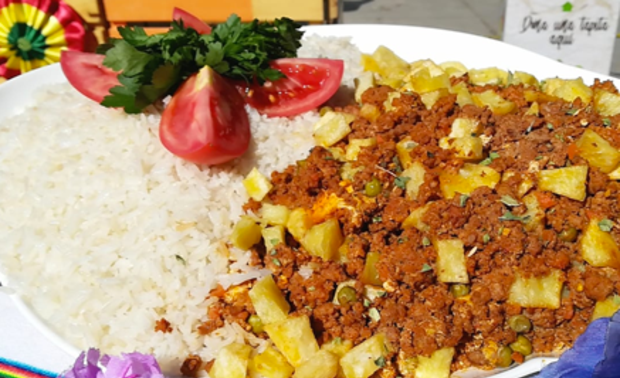
\includegraphics[scale=0.2]{revuelto-de-carne} 
    } & 
    \vspace{-1.8cm}            
    \begin{compactitem} 
        \begin{scriptsize}
            \item 1 kg carne molida
            \item 4 papas
            \item 2 zanahorias
            \item 3 huevos
            \item 1 taza arvejas
            \item 1 cucharilla de sal
            \item pizca de pimienta
            \item pizca de comino
            \item 2 dientes de ajo
            \item 1 cebolla
            \item 1 taza de arroz
            \item Aceite
        \end{scriptsize}
    \end{compactitem}&
    \vspace{-1.8cm}
    Primeramente freír las papitas así como si estuviera preparando papas fritas, la mejor manera de poderles escurrir el aceite sobrante es poner papel toalla o papel sabana en la fuente que utilizaremos para poner nuestras papitas fritas.

Seguidamente picamos nuestra cebollita en cubitos así como los dientes de ajo, estos dos juntos los ponemos a sofreír en una cucharadita de aceite caliente, una ves que estén trasparentes sacarlos en un platillo.

Poner a calentar nuevamente la sartén esta vez con dos cucharaditas de aceite, una ves caliente poner la carne y aplastarla con la cuchara de palito, condimentamos nuestra carne al gusto, con la sal, comino y pimienta, si quiere puede añadirle una pizca de orégano tb añadir la zanahoria en brunoise y arvejas , esperar a freír muy bien la carne.

Una vez frita, añadir la cebollita y el ajo, mezclar y también añadir las papas fritas, mezclar nuevamente hasta que los ingredientes estén uniformemente mezclados , entonces añadir los tres huevos cubriendo el sartén y todos los ingredientes.

Servir con arroz graneado.\\
    \hline

%---MARTES---%
    \pbox{20cm}
    {
        \rule{0pt}{3ex}\begin{large}\textbf{Martes}\end{large}\\ 
        \rule{0pt}{2ex}plato\\
        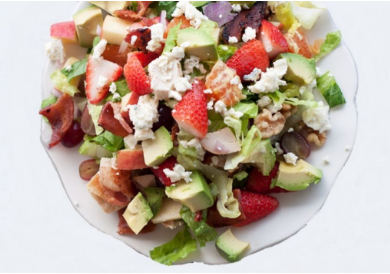
\includegraphics[scale=0.35]{ensalada-vegetal-con-carne} 
    } & 
    \vspace{-1.75cm}            
    \begin{compactitem} 
        \begin{scriptsize}
            \item x
        \end{scriptsize}
    \end{compactitem}&
    \vspace{-1.7cm}
    Receta.\\
    \hline

%---MIERCOLES---%
    \pbox{20cm}
    {
        \rule{0pt}{3ex}\begin{large}\textbf{Martes}\end{large}\\ 
        \rule{0pt}{2ex}plato\\
        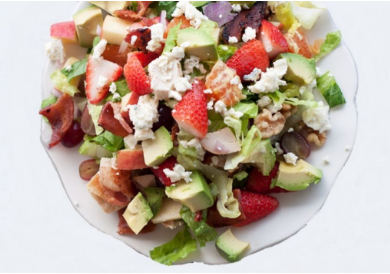
\includegraphics[scale=0.35]{ensalada-vegetal-con-carne} 
    } & 
    \vspace{-1.75cm}            
    \begin{compactitem} 
        \begin{scriptsize}
            \item x
        \end{scriptsize}
    \end{compactitem}&
    \vspace{-1.7cm}
    Receta.\\
    
\hline

%---JUEVES---%
    \pbox{20cm}
    {
        \rule{0pt}{3ex}\begin{large}\textbf{Martes}\end{large}\\ 
        \rule{0pt}{2ex}plato\\
        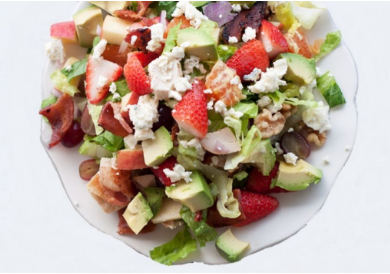
\includegraphics[scale=0.35]{ensalada-vegetal-con-carne} 
    } & 
    \vspace{-1.75cm}            
    \begin{compactitem} 
        \begin{scriptsize}
            \item x
        \end{scriptsize}
    \end{compactitem}&
    \vspace{-1.7cm}
    Receta.\\
    \hline

%---VIERNES---%
    \pbox{20cm}
    {
        \rule{0pt}{3ex}\begin{large}\textbf{Martes}\end{large}\\ 
        \rule{0pt}{2ex}plato\\
        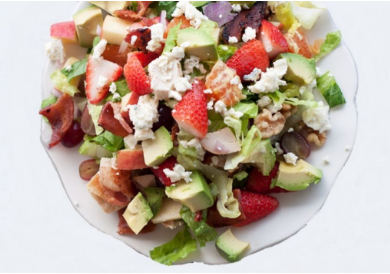
\includegraphics[scale=0.35]{ensalada-vegetal-con-carne} 
    } & 
    \vspace{-1.75cm}            
    \begin{compactitem} 
        \begin{scriptsize}
            \item x
        \end{scriptsize}
    \end{compactitem}&
    \vspace{-1.7cm}
    Receta.\\
    \hline

%---SABADO---%
    \pbox{20cm}
    {
        \rule{0pt}{3ex}\begin{large}\textbf{Martes}\end{large}\\ 
        \rule{0pt}{2ex}plato\\
        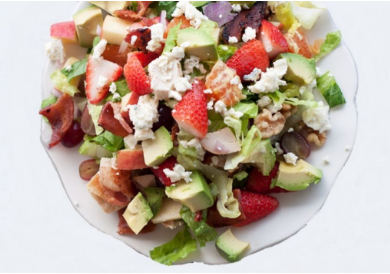
\includegraphics[scale=0.35]{ensalada-vegetal-con-carne} 
    } & 
    \vspace{-1.75cm}            
    \begin{compactitem} 
        \begin{scriptsize}
            \item x
        \end{scriptsize}
    \end{compactitem}&
    \vspace{-1.7cm}
    Receta.\\
    \hline
\newpage
\end{tabular}
\end{document}
